\section{管道中的有摩擦绝热流}

\begin{itemize}
    \item 理想气体 - 比热容为常数
    \item 稳态一维流动
    \item 绝热 - 没有热量传入或传出
    \item 摩擦因数$f$为此行数
    \item 不做功
    \item 竖直方向没有位移(重力不做功)
\end{itemize}

考虑如图\ref{24}的控制体

\begin{figure}[!ht]
    \centering
    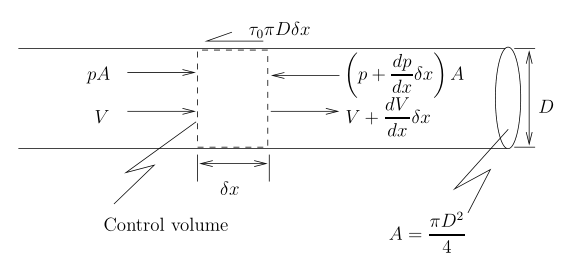
\includegraphics[width=\linewidth]{figures/24.png}
    \caption{控制体}
    \label{24}
\end{figure}

x方向的动量

\begin{gather*}
    p A-\left(p+\frac{d p}{d x} \delta x\right) A-\tau_{0} \pi \delta x D=\rho V A\left(V+\frac{d V}{d x} \delta x-V\right)\\ 
    d p+\frac{4 \tau_{0}}{D} d x+\rho V d V=0
\end{gather*}

其中摩擦因数的定义为

\begin{equation*}
    \tau_{0}=\frac{f \rho V^{2}}{8}
\end{equation*}


从而可以得到

\begin{equation*}
    \frac{d p}{p}+\frac{f \rho V^{2}}{2 D p} d x+\frac{\rho V d V}{p}=0
\end{equation*}

将第三项中的$\rho$,$p$,$V$利用马赫数代换可得

\begin{equation*}
    \frac{\rho V d V}{p}=\frac{\gamma M d M}{\frac{(\gamma-1) M^{2}}{2}+1}
\end{equation*}

类似地,第一项也可做类似的代换

\begin{align*}
    \frac{d p}{p}=\frac{-(\gamma-1) M^{2}+1}{\frac{(\gamma-1) M^{2}}{2}+1} \frac{d M}{M}
\end{align*}

代回x方向动量式可得

\begin{align*}
    \frac{f}{D} d x&=\frac{2\left(1-M^{2}\right) d M}{\gamma M^{3}\left(\frac{(\gamma-1) M^{2}}{2}+1\right)}\\ 
    &=\frac{2 d M}{\gamma M^{3}}-\frac{(\gamma+1)}{\gamma} \frac{d M}{M\left(\frac{(\gamma-1) M^{2}}{2}+1\right)}
\end{align*}

边界条件为

\begin{align*}
    M&=M_0\quad @x=0\\ 
    M&=M\quad @x=l
\end{align*}

对$x=0\sim l$积分,并带入$\gamma=1.4$,有

\begin{equation*}
    \frac{f l}{D}=\frac{5}{7}\left(\frac{1}{M_{0}^{2}}-\frac{1}{M^{2}}\right)+\frac{6}{7} \ln \left[\left(\frac{M_{0}}{M}\right)^{2} \frac{M^{2}+5}{M_{0}^{2}+5}\right]
\end{equation*}

如果令出口马赫数为1,可以得到$L_{max}$,当长度超过该限制时,流体会被限制

\begin{equation*}
    \frac{f L_{\max }}{D}=\frac{5}{7}\left(\frac{1}{M_{0}^{2}}-1\right)+\frac{6}{7} \ln \left[\frac{6 M_{0}^{2}}{M_{0}^{2}+5}\right]
\end{equation*}
